% !TEX root = ../master-thesis.tex

\begin{figure}
    \centering
    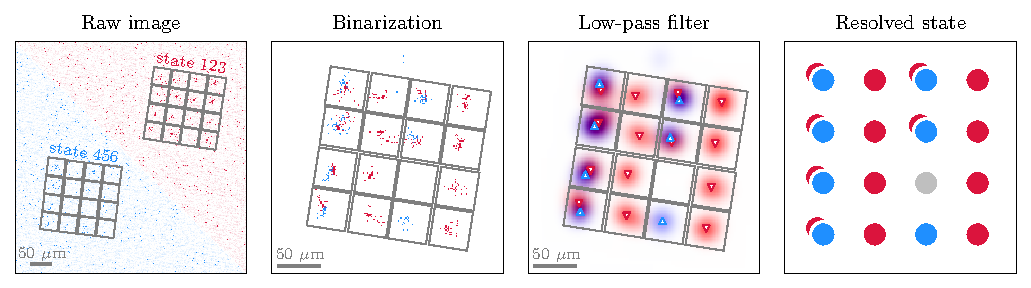
\includegraphics{fig-py/imaging-spin-resolved.pdf}
    \caption{
        \textbf{Spin-resolved single-atom imaging.}
        Spatially separated $\sigma_+$ and $\sigma_-$ fluorescence is imaged onto two distinct regions of the camera. The binarization step identifies photon counts above a threshold, followed by a low-pass filter to extract spatially localized signals. Final spin states are assigned based on relative signal strength in each channel:
        \raisebox{-1pt}{\scalebox{1.5}{\textcolor{ublue}{\textbullet}}} -- $\ket{1}$, 
        \raisebox{-1pt}{\scalebox{1.5}{\textcolor{ured}{\textbullet}}} -- $\ket{2}$, 
        \raisebox{-1pt}{\scalebox{1.5}{\textcolor{uhole}{\textbullet}}} -- no atom.
    }
    \label{fig:spin-resolved}
\end{figure}


\textbf{Single-shot spin resolution with spatial separation.}  
Spin detection is implemented through a single-exposure fluorescence measurement, where the emitted light from atoms in $\ket{3}$ and $\ket{6}$ is directed to different regions of the camera. This spatial separation is achieved using a polarizing beam splitter (PBS) after the imaging objective, which splits $\sigma^+$ and $\sigma^-$ components. In our geometry, atoms in state $\ket{3}$ produce fluorescence in the upper-right region of the frame, while those in $\ket{6}$ appear in the lower-left (see Fig.~\ref{fig:spin-resolved}). The system is calibrated so that each site in the tweezer array corresponds to two fixed analysis regions—one per spin channel.

\textbf{Filling detection.}  
For each tweezer site, the signal is integrated within two predefined ROIs, each capturing the fluorescence from one spin channel. The presence and identity of an atom is determined by comparing the signals from the two channels. If the signal in only one ROI exceeds a detection threshold, the corresponding spin state ($\ket{3}$ or $\ket{6}$) is assigned. If neither region contains sufficient signal, the site is identified as empty. If both channels yield strong and spatially localized peaks, this is interpreted as the presence of two atoms in different spin states at the same site.

\textbf{Fidelity estimation from single-atom preparation.}  
To characterize the performance of spin-resolved detection, we use deterministic state preparation. In these experiments, each tweezer contains an atom with a known spin state ($\ket{3}$ or $\ket{6}$) with approximately 95\% probability, as determined independently via fluorescence-based atom counting~\cite{dux_optical_2023}, see Fig.~\ref{fig:spillingadd}. Additionally, some choosen ROIs are intentionally left empty to provide ground truth data for evaluating false positive rates.

By applying the full detection pipeline to these experiments, we extract the rates of false positives (detecting an atom where none is present) and false negatives (failing to detect an atom where one exists). While the resulting classification accuracy depends on the overall filling fraction, the intrinsic detection characteristics (the false positive and false negative rates) are filling-independent. For a representative filling of 0.5, the resulting accuracy of spin-state assignment reaches 99\%. This performance level is sufficient for the current experiment stage.

\textbf{Implementation and contribution.}  
The complete processing pipeline for extracting spin-resolved occupancy data from camera images was implemented by the author. The classification algorithm builds on the same architecture used for unpolarized imaging but includes support for analyzing two spatially distinct fluorescence regions per site. The code is vectorized for efficient processing and can be extended to support additional spin channels or dynamic configurations.

